%%%%%%%%%%%%%%%%%%%%%%%%%%%%%%%%%%%%%%%%%%%%%%%%%
%%%%%%%%%%%% cap: installer %%%%%%%%%%%%%%%%%
%%%%%%%%%%%%%%%%%%%%%%%%%%%%%%%%%%%%%%%%%%%%%%%%%

\chapter{Creating an App Installer for the Platform}\label{cap:installer}
The platform solution proposed in this paper has harsh requirements when it comes to the folder hierarchy employed by the platform itself. All applications are stored at a specific location, said location can be hard to find for the end-user that is not experienced with navigating the Windows file system. To combat this lack of ease of use in less experienced users, this solution also implements another tool, an install wizard, to serve as a means to install applications automatically in lieu of doing it manually through the Windows File Explorer.


\section{Installer Architecture}
The installer is a Microsoft Foundation Class (MFC) type application. MFC was used to create the user interface for the installer and to make it easily exportable and compatible with all Windows platforms. The installer has 2 functions. It can install the platform itself, in any location the user chooses and it can install individual apps. The interface dialog allows the user to select individual applications to be installed via Check-Box Control type items. It then installs all of the selected applications using \textit{.bat} scripts that come with the installer itself that issue download requests to GitHub.

\begin{figure}[H]
  \centering
  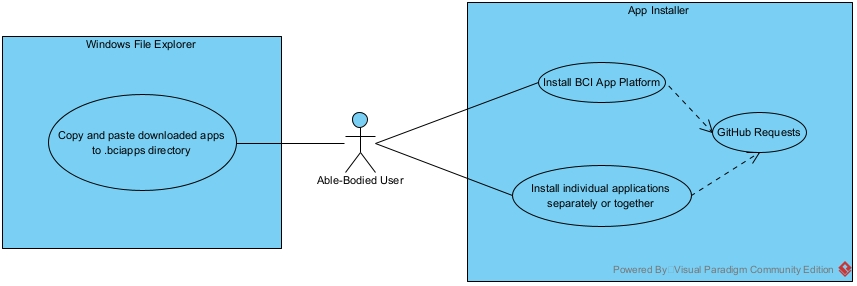
\includegraphics[width=1\textwidth]{Diagrams/Installer Use Case.jpg}
  \caption{Architectural Diagram}
\end{figure}



\section{Implementation Details}
The installer is a dialog-based MFC app built using the Visual Studio IDE and its visual C++ tools. The dialog and all controller logic are written in C++, while external \textit{.bat} files are used via system calls to issue the download and file manipulation commands inside the file system.

\subsection{MFC Application}
The MFC dialog consists of two parts, namely the platform installer and the application installer. Separated in their own group boxes, the parts each have their own controllers. The platform installation has an Edit Control to display the current installation path of the BCI App platform (which defaults to the user's Program Files directory each time the application starts) and two buttons, one labelled browse which serves as a way for the user to browse for his/her preferred directory and an install button, which calls the \textit{.bat} file that installs the platform. The second part, the app installer, consists of multiple check-boxes, each corresponding to its own application, from which one may pick the items they want and an install button that also uses a system call for the installation batch files. 

\subsection{Batch Files}
\begin{lstlisting}[language={[Sharp]C}, caption={c4.bat, the script file used for installing the Connect4 Game}, label={Script}]
@echo off
setlocal
set "url=https://github.com/DavidVuescu/BCI-Connect4/releases/download/v1.0.0-platform.1/app.zip"
set "outputPath=%TEMP%\app.zip"
set "extractTo=%userprofile%\Documents\.bciapps"
curl -L -o "%outputPath%" "%url%"
if errorlevel 1 (
    echo Failed to download file.
    exit /b
) else (
    echo File downloaded successfully.
)
powershell -Command "Add-Type -A 'System.IO.Compression.FileSystem'; [IO.Compression.ZipFile]::ExtractToDirectory('%outputPath%', '%extractTo%')"
if errorlevel 1 (
    echo Failed to extract file.
    exit /b
) else (
    echo File extracted successfully.
)
endlocal
\end{lstlisting}


In order to download and install anything, a batch file is used to send a download request to GitHub via the curl command. All compatible apps and the platform respectively have their binary files on separate GitHub releases, which can be fetched with the aforementioned commands. Each download is stored in the user's temporary files directory, inside a .zip file. The file is then extracted to its respective output path, either the .bciapps folder for applications or the user's preferred directory for the platform, after which the temporary download file is deleted so as to not consume space on the local user's disk[see listing 4.1]. In the case of an error, the program is simply not installed and the user can check the logs to see at which step of the process the installation failed.
\vspace{\baselineskip}\newline
When it comes to installing the applications the user selected via the checkboxes in the MFC dialog, a main installer.bat script is called alongside multiple arguments[see listing 4.2]. Each argument represents a code for a specific program to be installed. The installer.bat script loops through all arguments and checks whether they correspond to a compatible app inside the GitHub releases[see listing 4.3]. If it does, it executes the specific batch file for installing that application.

\begin{lstlisting}[language={[Sharp]C}, caption={Action Handler for the Install Apps button}, label={Script}]
void CInstallerDlg::OnBnClickedAppInstall()
{
	CString installerBatchFile = _T("installer.bat");
	CString arguments;

	UpdateData(TRUE);
	if (Connect4_Flag == TRUE) arguments += " c4";
	if (DaDa_Flag == TRUE) arguments += " da";
	if (BrainStompers_Flag == TRUE) arguments += " bs";
	if (Travelink_Flag == TRUE) arguments += " ta";
	if (NeuroArcade_Flag == TRUE) arguments += " na";

	CString command;
	command += _T(".\\"); command += installerBatchFile; command += arguments;
	int result = _wsystem(command);
	if (result == 0) {
		// Success // Do nothing
	}
	else {
		// Execution failure
		AfxMessageBox(_T("Could not execute installer.bat. Try redownloading the installer"));
	}
}
\end{lstlisting}

\subsection{Updatability}
As with any installer, as new applications roll out, the installer will become outdated, at which point the user can simply head to the GitHub repository for the installer and grab the latest release, containing the new applications. Furthermore, the installer tool is easily modifiable when the time comes for an update. Whenever a new application rolls out, a new checkbox can be added inside the dialog, a new batch script is added for curling the download URL and the modification is made inside of the Action Handler for the install button. While it may be more intuitive to run the batch files on their own or just manually download the app releases, this tool is a solution for the less technologically savvy people that want to use the platform quickly and don't want to bother with the technicalities of separate downloads or unknown scripts but instead would opt for a more user-friendly experience.

\begin{lstlisting}[language={[Sharp]C}, caption={Action Handler for the Install Apps button}, label={Script}]
@echo off
setlocal
echo Checking if .bciapps directory exists
call folder_validation.bat
for %%G in (%*) do (
    echo Active argument is: %%G
    if "%%G"=="c4" (
        echo Running Connect4 installer...
        call batch\c4.bat
    )
    if "%%G"=="da" (
        echo Running DaDa Painter installer...
        call batch\da.bat
    )
    if "%%G"=="bs" (
        echo Running BrainStompers installer...
        call batch\bs.bat
    )
    if "%%G"=="ta" (
        echo Running Travelink Around installer...
        call batch\ta.bat
    )
    if "%%G"=="na" (
        echo Running Neuro Arcade installer...
        call batch\na.bat
    )
)
echo All batch files executed.
pause
\end{lstlisting}



\section{Graphical Interface}
\begin{figure}[H]
    \begin{minipage}[c]{0.45\linewidth}
      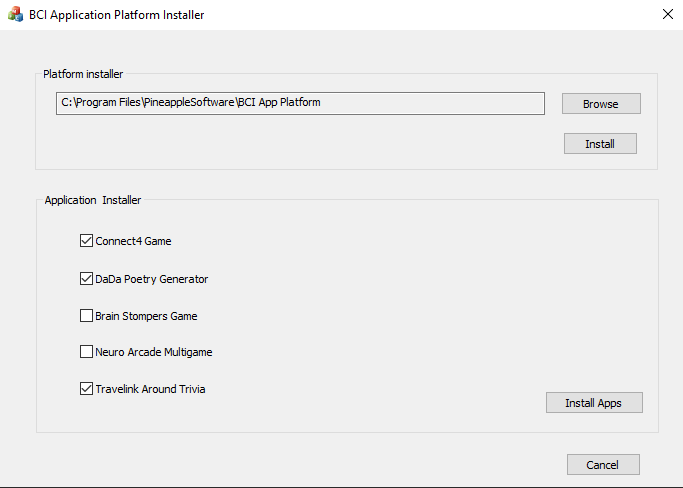
\includegraphics[width=\linewidth]{Graphics/Installer GUI.png}
      \caption{Installer Dialog Window}
      \end{minipage}
    \hfill
    \begin{minipage}[c]{0.45\linewidth}
      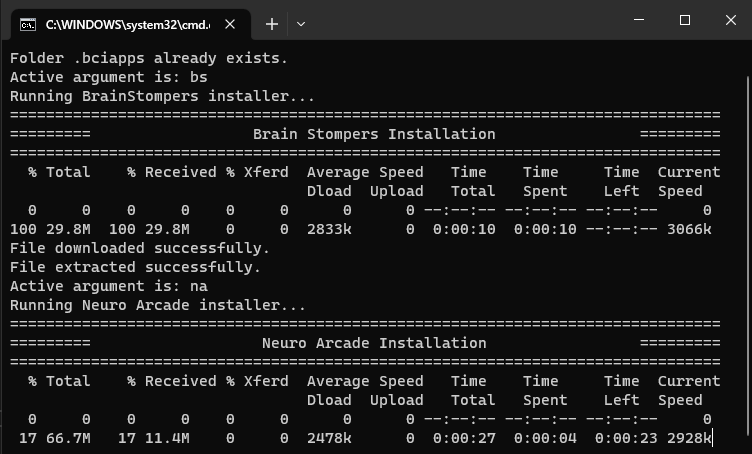
\includegraphics[width=\linewidth]{Graphics/Installer Terminal.png}
      \caption{Installer Terminal Window}
  \end{minipage}%
\end{figure}
The upper part of the installer is reserved for the platform installation, while the lower is used for the different applications' checkboxes. Alongside the main dialog, a terminal window opens each time a user presses an install button for logging purposes.

